\chapter{Indledning}
\section{Projektformulering}
Mange ældre har i dag svært ved at åbne deres vinflaske, da de ikke har den fornødne styrke til selv at trække korkproppen ud af vinflasken. Derfor ville det være ideelt for dem, at have en løsning hvor åbningen af vinflaskerne bliver automatiseret.

For at få den optimale oplevelse ud af en vin, skal den åbnes rettidigt så den iltes før indtagelse. Iltningstiden kan variere fra vin til vin, og derfor kan mange uerfarne vindrikkere have svært ved at ilte deres vin korrekt. Mange glemmer at åbne vinen i god tid, og opnår derfor ikke den optimale oplevelse. Det kan derfor være ideelt, hvis denne proces også automatiseres.

\subsection{Projektdefinition}
Ud fra ovenstående problemstillinger skal der fremstilles et produkt som skal automatisere vinåbning og iltning, samt hvis muligt  oprette et netværk hvor vindrikkere og forhandlere kan sættes i forbindelse med hinanden. Produktet har følgende systemkrav:

Systemet: \begin{itemize}
	\item Skal trække korkproppen ud af en vinflaske, og ilte vinen korrekt. I denne proces indgår aktuator, sensor, PSoC, Devkit og motor.
	\item Skal betjenes via Devkit 8000, hvor der er installeret Linux.
	\item Skal meddele brugeren når vinen er klar.
	\item Skal kunne indstilles til at trække korkproppen ud til et givent tidspunkt.
	\item Skal holde vinflasken fast under udtrækningen af korkproppen.
	\item Skal detektere afstanden fra toppen af flasken til åbningsmekanismen.
	Skal kunne bortskaffe vinpropper efter åbning.
	\item Skal kunne give status for vinåbningsprocessen.
	\item Skal kunne åbne vin hurtigt, når situation kræver det.
	\item Skal have et grafisk brugerinterface til betjening af vinåbningen.
	\item Skal give brugeren mulighed for at indstille klokken på et indbygget realtidsur.
	\item Skal have et grafisk brugerinterface til betjening af vinåbningen.
	\item Bør have en sikkerhedsmekanisme til forebyggelse af personskader.
	\item Bør ud fra vinens type kunne ilte vinen korrekt.
	\item Kunne hvis muligt måle vinflaskens temperatur.
	\item Kunne hvis muligt fjernbetjenes med en mobil applikation, således at brugeren har mulighed for at ændre på et evt. åbningstidspunkt.
	\item Kunne hvis muligt tilkobles en database med information om forskellige vine og deres iltningstid, så det er muligt at automatisere iltningsprocessen ud fra de enkelte vine.
	\item Kunne hvis muligt forbindes til et online socialt netværk, så vindrikkere kan give anmeldelser af forskellige vine.
	\item Kunne hvis muligt give bruger mulighed for at bestille vine direkte fra en forhandler.
	\item Kommer ikke til at kunne tilsluttes det danske el-net.
\end{itemize}

\begin{center}
	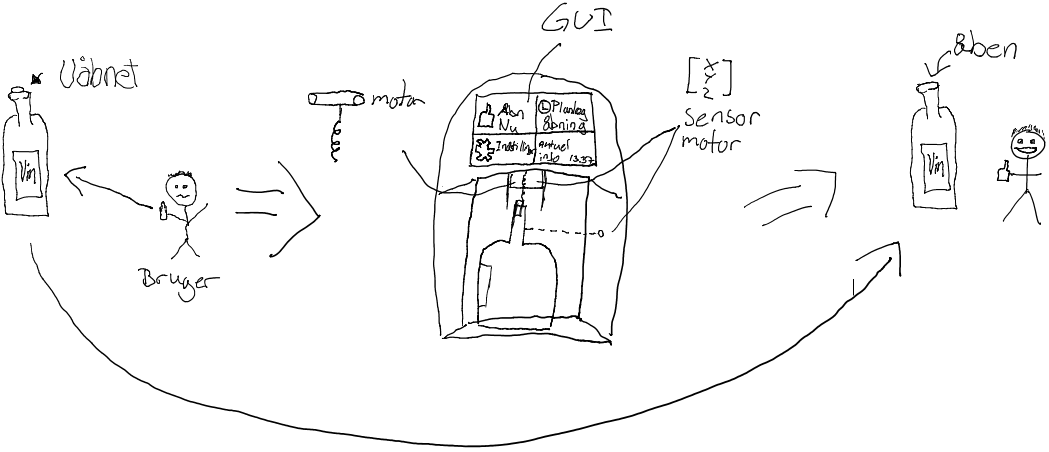
\includegraphics{WinePrep_realistisk.png}
\end{center}
